% This is a template designed by Maarten J. Waterloo for BSc and MSc
% students at the Faculty of Earth and Life Sciences, Vrije Universiteit
% Amsterdam, adapted to the University of Freiburg by Carsten F. Dormann. 

\documentclass[11pt,twoside,a4paper,final]{report}
% We define a two-side report on A-4 paper in final quality using a
% point size of 11 for the text. Other possibilities are {book},
% {article}, etc.

% A % sign indicates that text is commented out and will not appear in
% the document. Use \% if you want to indicate a % symbol in the text,
% thus 10\% will become 10%...

% We need to include some packages for layout and style. We do this
% below using the \usepackage command. A short explanation for each
% package is included.

\usepackage{amsmath}   % If you are going beyond the most basic level
                       % of displayed equations, you will benefit from
                       % using the amsmath package that plugs into
                       % LaTeX. This package has lots of useful
                       % features for multi-line equations, compound
                       % symbols, even commutative diagrams! Allows
                       % use \text in equations	

\usepackage{booktabs}  % booktabs is to enable the easy production of
                       % tables such as should appear in published
                       % scientific books and journals. What
                       % distinguishes these from plain LaTeX tables
                       % is the default use of additional space above
                       % and below rules, and rules of
                       % varying`thickness'.

\usepackage[top=3cm, bottom=3cm, outer=2.5cm, inner=3.5cm]{geometry}  
					   % formating the page margins

\usepackage{graphicx}  % The graphicx package implements LaTeX
                       % support for including graphics files,
                       % rotating parts of a page, and scaling parts
                       % of a page. The package depends on having a
                       % DVI driver that can produce these effects.
                       
\usepackage[hidelinks, breaklinks]{hyperref} %This package will make links in PDF
                       % documents to your figures, references, etc.
                       % hidelinks removes the boxes around the hyperreferenced items
                       
\usepackage[utf8]{inputenc} % Hard to explain: Define here the text encoding 
					   % used by your computer; on Linux typically utf8, on 
					   % windows ansinew and on mac often latin1;
					   % ideally, the whole world would use utf8
					   % important for öüäß (Umlaute)

\usepackage[ttscale=0.875]{libertine} % Use a nice serif font! Alternatives:
					   % times, palatino, ... 
					   
\usepackage{makeidx} % use this package to make an index
                       % of keywords, you have to follow this by the
                       % \makeindex command 
\makeindex             % Create the index file        

\usepackage{natbib}    % Provides a style with author-year and
                       % numbered references, as well as much detailed
                       % of support for other bibliography
                       % use. Provides versions of the standard BibTeX
                       % styles that are compatible with natbib,
                       % plainnat, unsrtnat,
                       % abbrnat. The bibliography styles produced by
                       % custom-bib are designed from the start to be
                       % compatible with natbib.
  %bibtex related settings-------------------------------------------
  \def\bibfont{\small} % change font size to small
  %\renewcommand{\bibfont}{\footnotesize}
  \renewcommand{\bibsep}{5pt}
  \bibpunct{(}{)}{;}{a}{}{,} % change square brackets to round ones, separators between authors to ; and so forth
                      
                       
\usepackage{rotating}  % The rotating package implements three
                       % environments within which in-line figures,
                       % tables, and captions can be rotated by an
                       % arbitrary number of degrees. Two additional
                       % environments allow rotation of floating
                       % objects, which are typeset alone on separate
                       % pages.

\usepackage{wrapfig}   % allows text to flow around a figure               


% The \raggedbottom declaration makes all pages the height of the text
% on that page. No extra vertical space is added.
\raggedbottom

%----------------------------------------------------------------------------
% Allow more floating material on text pages:
\renewcommand\floatpagefraction{.9}%
\renewcommand\topfraction{.9}%
\renewcommand\bottomfraction{.9}%
\renewcommand\textfraction{.1}%
\setcounter{bottomnumber}{4}%
\setcounter{topnumber}{4}%
\setcounter{totalnumber}{4}%


%----------------------------------------------------------------------------
				% here the content starts !		
%----------------------------------------------------------------------------
% Define title and authors
\def\maintitle{On the intersection of desirability, reachability and sleeping disorder: the role of the final thesis in the maturation of a student}
%\def\subtitle{Subtitle...}
\def\authors{Whathave I. Learned }
\def\supervisor{Supervisor: Prof. Dr. Irene Knowitall, Department of Irreproducible Affairs}
\def\cosupervisor{Co-supervisor: Prof. Dr. Jörg Noinput, Department for the Investigation of the Unknown}
\def\year{Freiburg, May 2014}
\def\course{Bachelor thesis  (Student ID 450100) \\submitted to \\the Faculty of Environment \& Natural Resources \\ at the Albert-Ludwigs-University Freiburg}

% Start the document
\begin{document}

% Make some shortcuts for writing units and chemical species
% You can add your own here...
\newcommand{\mgl}{mg l$^{-1}$}
\newcommand{\mmoll}{mmol l$^{-1}$}
\newcommand{\meql}{meq l$^{-1}$}
\newcommand{\muscm}{$\mu$S cm$^{-1}$}
\newcommand{\water}{H$_2$O}
\newcommand{\kion}{K$^+$}
\newcommand{\naion}{Na$^+$}
\newcommand{\caion}{Ca$^{2+}$}
\newcommand{\mgion}{Mg$^{2+}$}
\newcommand{\clion}{Cl$^-$}
\newcommand{\nitrate}{NO$_3^-$}
\newcommand{\nitrite}{NO$_2^-$}
\newcommand{\nhion}{NH$_4^+$}
\newcommand{\hcoion}{HCO$_3^-$}
\newcommand{\hardness}{Ca$^{2+}$ + Mg$^{2+}$}

% Pagestyle of numbering, options are plain (Just a plain page number), empty (empty heads and feet - no page numbers), 
% headings	(puts running headings on each page), and myheadings (You specify what is to go in the heading with the 
% \markboth or the \markright commands.
% No numbering on title page, so we use empty here...
\pagestyle{empty}

%-- french title page (r) ------------------------------------------------
% Include the university-logo at the bottom of the page
\begin{figure}[h]
  \begin{flushright}
    \vspace{-2cm}
    
\includegraphics[width=4cm]{images/ufcd-logo-e1-a4-color} %ALU_longlogo}
  \end{flushright}
\end{figure}

\begin{center}
  {\huge\bfseries\maintitle\par}
  \vskip 2em%
%  {\Large\bfseries\subtitle\par}
%  \vskip 2em%
  {\Large\authors\par}
   \vskip 2cm%
  {\course\par}
  \vskip 1em%
   \begin{figure}[h]
     \begin{center}
       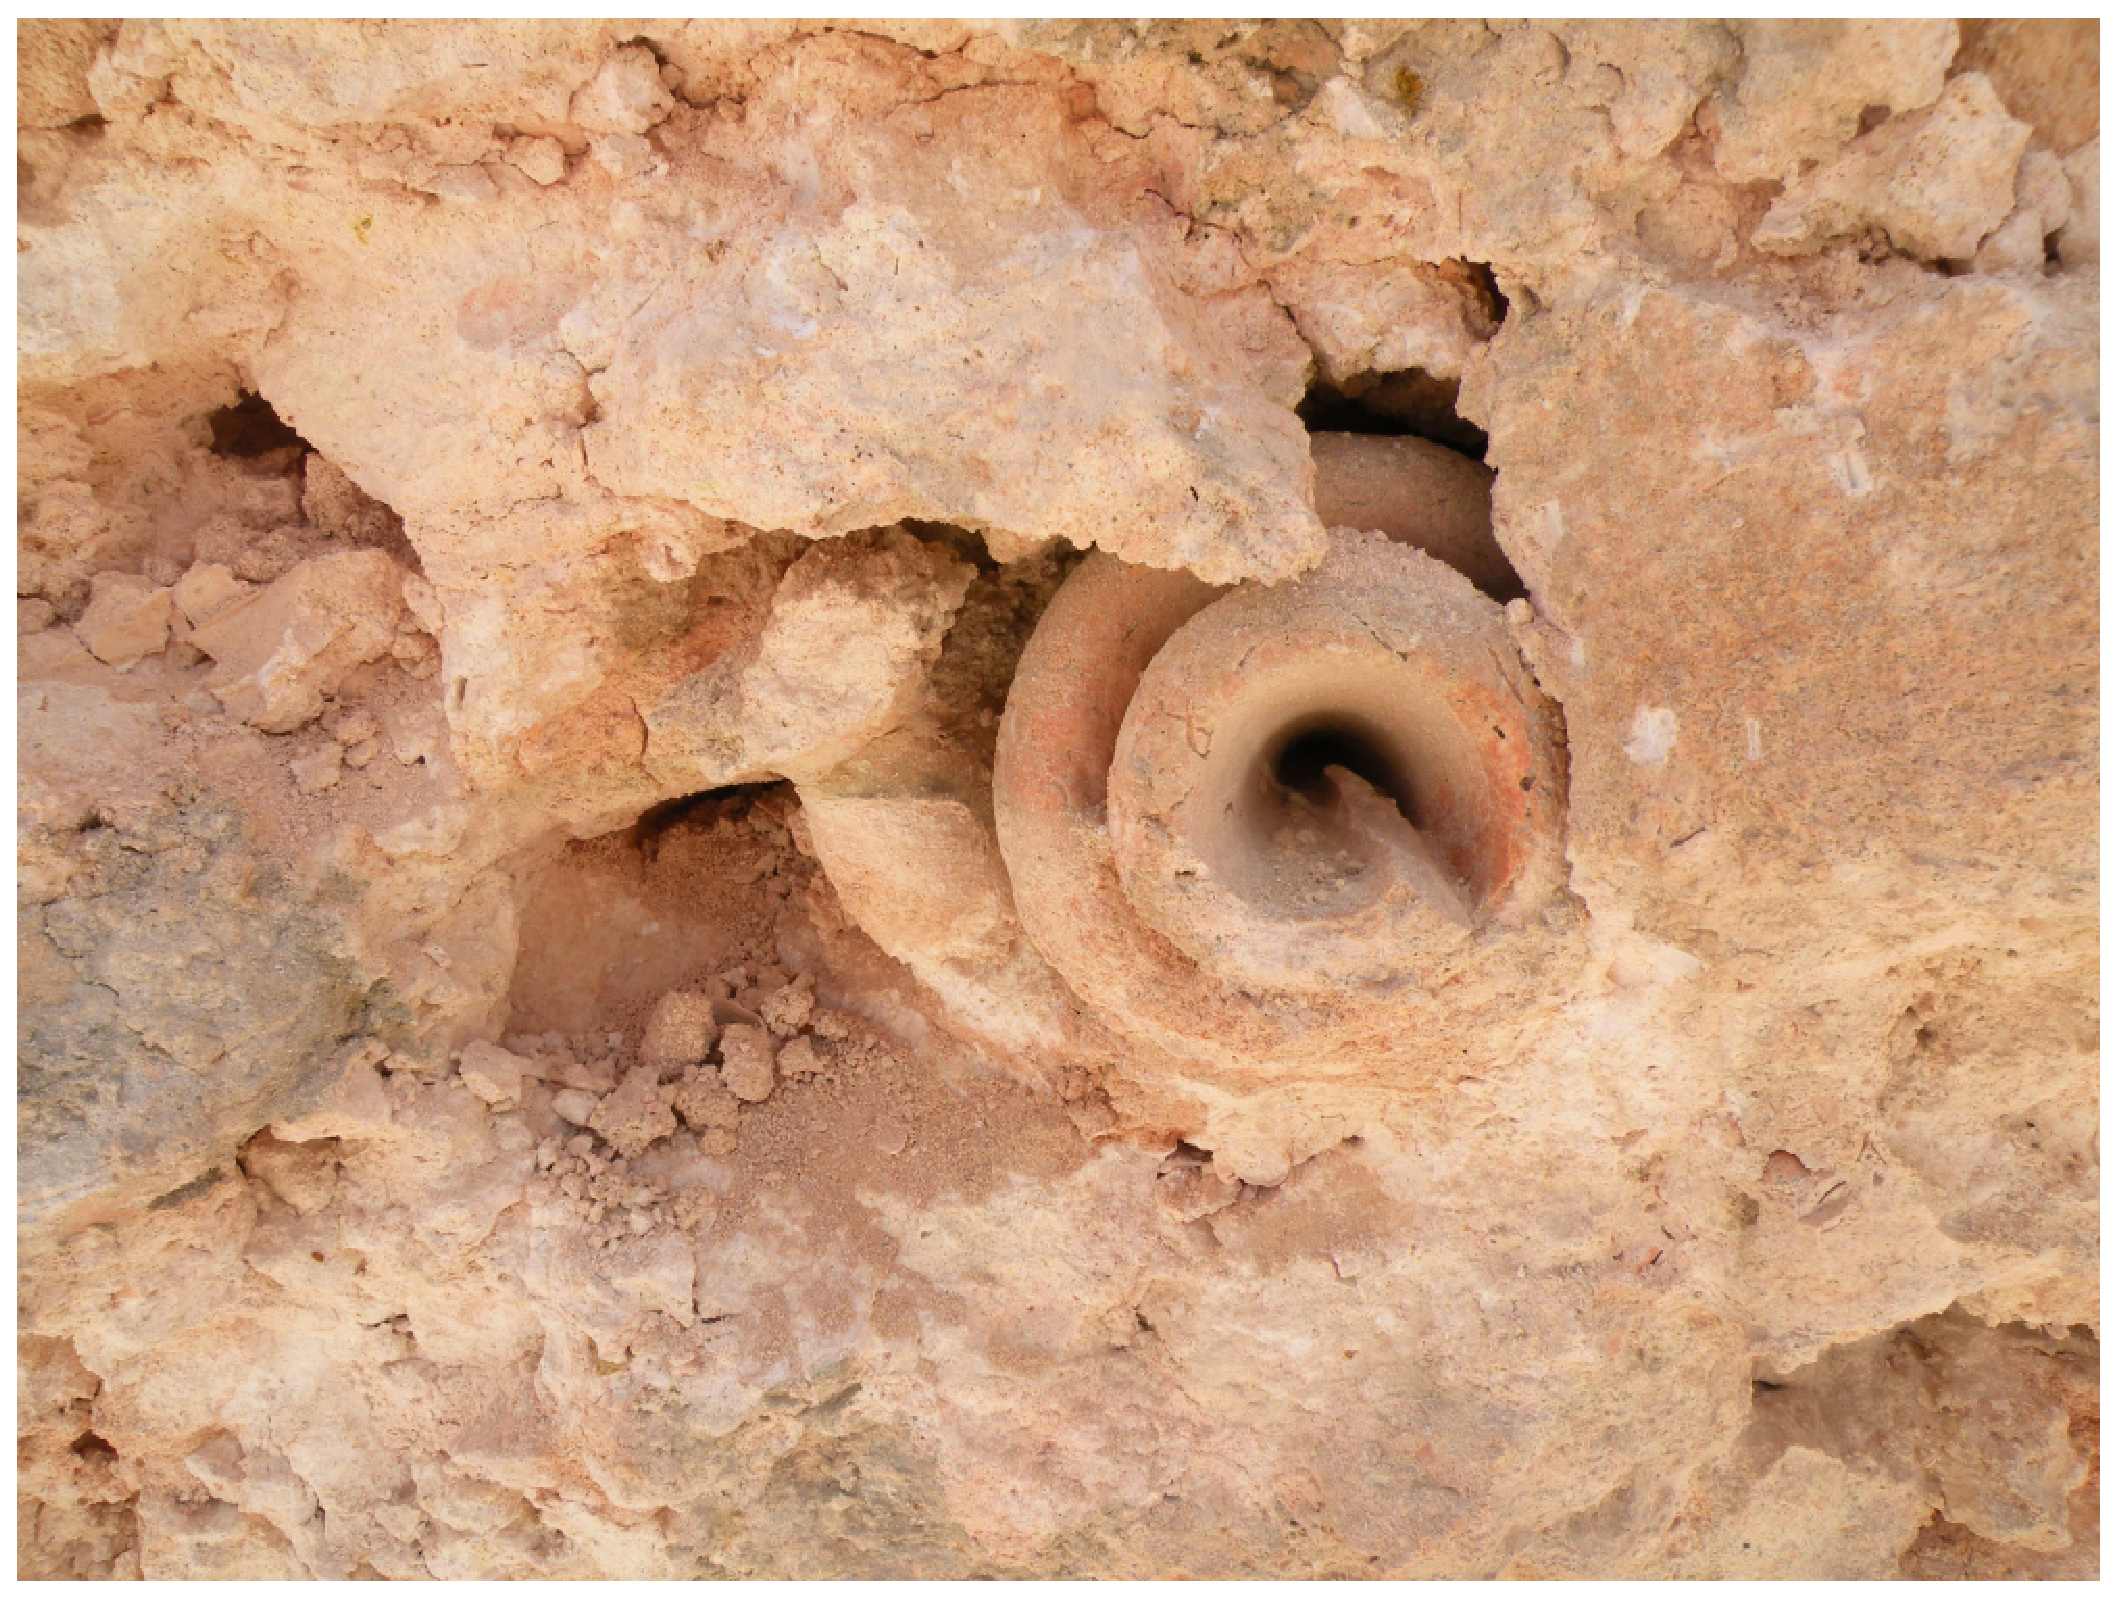
\includegraphics[width=10cm]{images/bsc-fossil}
    \end{center}
  \end{figure}
 % \vskip 2em%
\end{center}
  {\supervisor \\  \cosupervisor \\
  \flushright \year \par} 

\newpage
% If you have a photo on the titlepage, you can add a short
% explanataion here 
Cover photograph: Example of a fossil in a reef. Source: somewhere from the internet ...

\newpage

% Page numbering, options are arabic (Arabic numerals), roman	(Lowercase Roman), Roman (Uppercase Roman)
% alph (lowercase letters) and Alph (Uppercase letters)
\pagenumbering{Roman}
\pagestyle{plain}

% Include table of contents
\tableofcontents

% Remove the % in front of the command below to include a list of tables:
%\listoftables

% Remove the % in front of the command below to include a list of figures:
%\listoffigures

\newpage
% Use arabic numbering throughout the text
\pagenumbering{arabic}


\frenchspacing % this reduces the width of a space after a "." French spacing is also the default in most of the world, and even in the US print media.


% Include an abstract of your report
\abstract{
Place your abstract text here

Attention! In \LaTeX{ }you \textbf{use an empty line to create a new paragraph}. This leads to the first line of the new paragraph being indented (apart from the first of a section). This is intentional and nice! If you disagree, you can redefine the settings (\texttt{parindent} and \texttt{parsep}\footnote{As demonstrated here:  \url{https://texblog.org/2012/11/07/correctly-typesetting-paragraphs-in-latex/}}), but PLEASE NEVER use the double-backslash to end a paragraph! That is bad style and can get you into all sorts of incompatibility problems. 

So: no \textbackslash\textbackslash~ to end paragraphs!


And while we are at it: \LaTeX{ }has a few notational standards differing from ordinary writing programms. For example, \textbf{quotation marks} are typically \emph{not} correctly displayed! Although tedious, use \`{}\`{} (i.e. backticks) and '{}' (i.e. apostrophes) to achieve ``this'' (i.e. typographically satisfactory quotation marks).\footnote{\url{https://www.maths.tcd.ie/~dwilkins/LaTeXPrimer/QuotDash.html} For German text, use \`{}" and '{}", i.e. with the normal quotation mark: \url{https://tex.stackexchange.com/questions/38965/problem-with-using-quotations-in-german-document?rq=1}.} 

When you cross-reference a figure, you don't want the number to be separated from the word by a new line, but rather keep ``Fig.'' and ``3'' together. To do so, \LaTeX{ }offers a \textbf{non-breakable space}, using the tilde ($\sim$), like so: \texttt{Fig.{\raise.17ex\hbox{$\scriptstyle\mathtt{\sim}$}}\textbackslash  ref\{fig:studysite\}}. (A breakable forced space would simply be two curvy brackets around an empty space, i.e. \{\textvisiblespace \}, as I used every time after the \texttt{\textbackslash LaTeX}-command above.)

If you want to \textbf{display code} (of virtually any programming language, including R, Matlab, C/C++, Java, Python, \LaTeX), you should have a look at the listings package.\footnote{\url{https://en.wikibooks.org/wiki/LaTeX/Source_Code_Listings}, \url{https://texfaq.org/FAQ-codelist}}

} 



% Start with the first chapter
\chapter{Introduction}
% With \label you can define a crossreference so that you can refer
% to this chapter later in the text by using Chapter~\ref{ch:background}
\label{ch:introduction}


Start your introduction here...

Possibly cite some work of others, too \citep{Adiku.ea:1995:USO}. To do so, you have to fill a file (the bibliography, recognisable by the \texttt{.bib} ending) with appropriately formatted references. It would be daft to not use BibDesk or JabRef or other software to manage your references and produce this file for your. Then, you cite the references, and the \textbf{natbib} package allows you flexibility (with/out parentheses, only the year, etc). The actual style of the bibliography in your thesis is determined by the command \texttt{bibliographystyle}, and there are only few defaults. The main differences are between author-year styles (e.g. apalike) and numbered (e.g. ksfh\_nat). Thousands of styles float the internet, recognisable as \texttt{.bst}-files, and typically every journal has a different one, every book series re-invents the styles, and you can spend years optimising what is, essentially, not so super important.

\begin{boxmd}
	\textbf{Bibliography settings}\\
	Just like in any other writing software, references are collected and managed in a dedicated programme (a reference manager, e.g. Zotero, BibDesk, JabRef, ...). This results, for \LaTeX, in a \BibTeX\/ file, recognisable by the \texttt{.bib}-extension, with a readable but very structured content. When you import a publication into the reference manager, the title may be unformatted; italics (e.g. species names) and capitalisation (countries, Names) may well be lost, and you need to put them back in. 
	Eventually, your \BibTeX-file should have entries that look like this:\\
	%
	\begin{footnotesize}
	\begin{ttfamily}	
	@article\{Dormann1997,\\
	Author = \{Dormann, Carsten F\}, \\
	Journal = \{Zeitschrift f\{\textbackslash"u\}r \{\textbackslash"O\}kologie und Naturschutz\},\\
	Pages = \{26-\.-36\},\\
	Title = \{Sandrohr (\textbackslash emph\{\{C\}alamagrostis epigejos\} (L.) \{R\}oth) in \{T\}rockenrasen des \{B\}iosph\{\textbackslash "a\}renreservates \{S\}chorfheide-\{C\}horin: \{B\}estandsstruktur, \{\textbackslash"o\}kologische \{A\}uswirkungen und \{P\}flegemassnahmen\},\\
	Volume = \{6\},\\
	Year = \{1997\}\\
	\}
	\end{ttfamily}
	\end{footnotesize}\\
	You will note that all capital letters in the title need to be surrounded by braces ``\{\}'' to prevent conversion to lower case. Italics, such as the species name here, need to be explicitly emphasised. Diacritic symbols may require special representation, although not if you have set your input encoding correctly (see preamble of this document).
	
	Of course you can use the more flexible Bib\LaTeX instead of \BibTeX, and of course there some small things to know about the entry types in either. But this should get you started with papers. For books, there is \texttt{\makeatletter @\makeatother book} and for chapters there is \texttt{\makeatletter @\makeatother incollection} (do not use \texttt{\makeatletter @\makeatother inbook}, which does not allow you to specify the editors). I try to squeeze everything into these three types of references.
	
	Pay attention to correct capitalisation of your references. Typically, and preferably, Book Titles should be in capitals, as should Journal Names, while journal publications should be lower case, as should be the titles of book chapters. Once your \texttt{.bib}-file is set up correctly, this is all taken care of by the bibliography style of your choice.
	
	Finally, do \textbf{not} print both DOI and URL in the bibliography, they are typically near-identical. Check the internet for how to suppress URL in this case (although I think the style used here does that automatically, at the expense of also suppressing the DOI).
\end{boxmd}



To add florish, you can use so-called ``fleurons'' to separate paragraphs of the introduction (or discussion) that are really different but have no separate section titles. In novels these are typically changes of scenes within a chapter. The most common fleurons are leaves (\adfhangingflatleafright), asterisks (\adforn{5}) or wiggles (\adforn{19}),
but I like fleurons related to the topic of your work, so for one on elephants you could do this: 

{\centering
	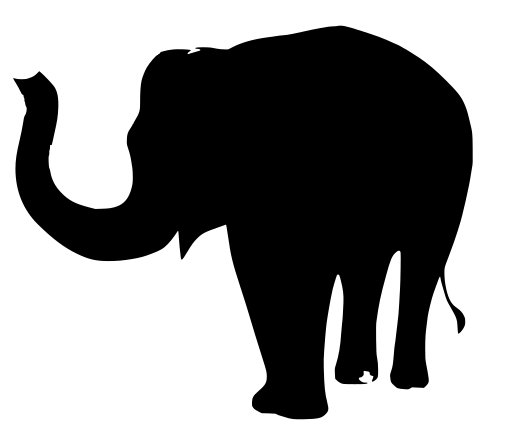
\includegraphics[width=0.5cm]{images/elephant.png}
	
}
%Note the empty line: without it will not yield what we want!!

\noindent After such a large gap, you should continue without indented first line! Most supervisors may find such embellishments distracting, unscientific bauble (and they are, but hey, life is also fun). So better check with them before submission!

%\clearpage
%
%{\Large \textbf{Want to write your BSc or MSc thesis under my supervision? Read this first!}}

\bigskip
\noindent For those few people whose work will be assessed by me (Carsten Dormann, Uni Freiburg), here are some general but personal thoughts on what makes a great piece of science.

I think of science as composed of (at least) two parts: \emph{handcraft} and \emph{intellect}. The handcraft is important to ``get things right''. It is what you (hopefully) learn to a large extent at university, from designing experiments, to various methods of collecting data, lab work, plotting, analysing, to writing it all up in a standardised (and thereby easily accessible) way. Handcraft includes issues such as reproducibility and publishing ethics.

\emph{Intellect} is where the actual ``science'' happens, it is the progress in understanding the world, the increase in knowledge, the broadening of the mind and the trimming down on possible ways things could interact. I see handcraft as the stuff that every baker has to do, too: get the dough set up tastily, have the right ingredients, the right temperature in the oven, a clean working surface, safe working conditions, etc. The baker also should work reproducibly (from day to day) and ``publish'' (read: sell) his/her results.

It is harder to describe what is a ``good'', intellectual science contribution. As first approximation, I think science is stuff that will still be correct in, say, 500 years. I am not against short-term benefits of science, don't get me wrong, but those are largely engineering, i.e. applying in exceedingly smart ways our \emph{current} knowledge to problem solving. There is no demeaning in calling an activity ``engineering'': it is of vital importance for all our societies, our everyday life and our future. It is (or at least can be) highly creative and responsible, challenging and demanding the highest level of intelligence. During engineering projects, a lot of still-valid-in-500-year-stuff is being produced, i.e. science is ``done''. 

In a science degree, however, this is not the typical approach to ``doing science''.\footnote{I am aware that many politicians think that this is how science \emph{should} be done, that science is only to directly benefit the university, the society, the economy. Also, I am aware that some thinkers (in a wider sense of the word) suggest that most actual science progress is serendipitous, and hence engineering is all we need. I just happen to disagree, possibly for selfish, stupid or conservative reasons.} 
Here, understanding the inner workings is the goal, not an application, or problem solving activity, however worthy. And the key (only?) approach that has over a few centuries proven useful for ``doing science'' is ``the Scientific Method''. This is based on a theoretical understanding, from which we derive hypotheses that are then tested.\footnote{If unfamiliar with the Scientific Method, do read it up on Wikipedia or alike. By all means, also read the criticism levelled at this approach. Keep in mind, though, that ``the hard sciences'' (physics, chemistry and friends) use this approach as their bread-and-butter epistemology. Don't reject it just because you don't like it or find it wanting for some reason. It has a very good track record!}

For a BSc, MSc or other scientific work, this has substantial consequences. First, it requires the author to lay out the \textbf{theory}. Without theory (or model or process understanding) one cannot derive (``deduce'') hypotheses. Into how much detail of said theory one has to go depends on the actual hypothesis to be tested. If your theory is that the moon was formed from the same material as the earth, and you want to test the hypothesis that thus the mineral composition is the same for both celestial bodies, well, I guess you can keep it short and focus on \emph{which} minerals you want to investigate and \emph{why those}. On the other hand, I would like to know what makes you want to test such a theory, and while you can simply cite some authority on the subject, it is better practice to recount the actual arguments and facts so far.

Next comes the formulation of hypotheses that could be used to test this theory. Obviously a good theory makes an awful lot of statements, so we cannot, in a lifetime, test all of them. Typically the department where you work determines which hypotheses you will test. (This sounds like a really stupid reason, but in real life a lot of things are really stupid.) And, luckily, it is actually not such a bad reason. Your department (or your supervisor's department) will have experience in a certain way of hypothesis-forming and -testing, will have certain lab facilities, data, collaborations, expeditions and so forth. Hence even though the best way to test a theory may be a specific hypothesis, it will simply be out of reach (think: explode a planet, fly at 90\% the speed of light or speak fluent Khoisan). It is IMHO extremely important to be aware of these constraints and limitations! You should be able to answer to any journalist with the best possible way to test a theory, and why you couldn't use that approach. Don't even pretend that your approach is anywhere near optimal or even decent. We all are aware of how limited our possibilities are, and grandiousing our ways (if that is a word) is silly, self-deceiving and transparently wrong.

It is very useful, and hard, to go through all the possible outcomes of your hypothesis-testing and work out \emph{in advance} what you learn from it. If there are 120 ways why you don't get a positive finding, well, then you don't actually learn much from such a negative finding. Since most easy hypotheses have been tested over the last few hundred years of science, you will most likely find your hypothesis rejected. That is, in itself, fine. But it is only fine if you still learn something from it, if it narrows down possibilities. If, say, you find that a higher plant species richness does \emph{not} lead to a higher monkey density in a Madagascan forest, well, there may be hundreds of reasons why it didn't. This is no intellectual progress. It is not the lack of a positive finding, it is the lack of a \emph{conclusive} negative finding that will bother reviewers! If, in contrast, you visited one of the 10 candidates for a meteorite impact crater responsible for the \href{https://en.wikipedia.org/wiki/Permian%E2%80%93Triassic_extinction_event}{Permian-Triassic extinction event}, 
and you found the isotop composition not to be consistent with this site being ``it'', well, then we actually learned something (for the next 500 years)!

Where, you may ask, was the ``intellect'' in the last example? Good point! That was indeed handcraft research, not intellectual science. Note that this is a document for BSc and MSc theses, not the Noble Price. And for a, say, MSc thesis I would be very happy to read the theoretical reasoning, the derivation of what to expect if this site \emph{were} the impact crater, to see the discussion (and quantification) of the uncertainty of the isotope measurements and thus the strength of the rejection of this site. It would, to me, demonstrate that you had worked scientifically. Would you get full marks? Alas, no. The missing bit was the curiousity driven, creative advancement to theory. Not everybody will be able to do that. In fact, I doubt that I have made substantial contributions to this still-valid-in-500-years-stuff (and I certainly never got full marks after leaving school). But that is exactly what a full marks means: exceptional, outstanding, dazzling! And few of us are geniuses worthy of full marks, sorry. You can become a good scientist, contributing to advancing the work on the still-valid-in-500-years-stuff even without being a genius (at least that's what I keep telling myself).

So I guess what I'm saying is: Don't expect exceedingly good marks from me.



\chapter{Methods}
\label{ch:methods}
You may want to start with a few, brief sentences of what you actually did, before going into the details over the next sections.

\section{Site}
\section{Species}
 Remember that Latin species names are set in italics, and only the genus name is capitalised: \emph{Lacerta viridis}.
\section{Statistical Analysis}

  Describe the methods and measurements that you used here.

\begin{itemize}
\item Units (m, kg, s) should be separated by a space from the value, except for \% and ° (or '' and ' for geographical coordinates): ``We weighed all bolders in the vicinity of the south pole ($-90$°N $0$°E) to an accuracy of 5 g, i.e. to an accuracy below 0.1\%.''

\item Write ``a 2 km $\times$ 2 km grid'', and not ``a 2 $\times$ 2 km grid'' (because the units need to be correct).

\item In the text, you can use \texttt{\textbackslash textsubscript} instead of the math mode (\$ ... \$) like so: CO\textsubscript{2} vs CO$_2$.

\item In equations, text should be displayed as text, not as mathematical symbols: $n_\text{total}$ or $df_\text{residuals}$, not $n_{total}$ or $df_{residuals}$.

\item Note that numbers may look different (are of different size!) in text and math mode, as does the minus: -2.0°C vs $-2.0$°C. Use the math mode consistently for numbers when these indicate an actual mathematical numeral, not an English word (such as 1776 or chapter 5, where you should use the text mode). For units and number representation you can use the package \textbf{siunits} for maximal standardisation: \num{2.34 x 5.67} or $\SI{-2}{\celsius}$. I regard this as overkill in most situation, though.
\end{itemize}  
 
 

\chapter{Results}
\label{ch:results}

Describe your results here...


\chapter{Discussion}
\label{ch:discussion}

Try to write introduction and discussion in a way that the reader doesn't really require methods and results. To do so, you have to use the first (few) sentences of the discussion to recapitulate your findings.

Discuss your results here, ideally structured into various sections, of which one is:


\section{Conclusions}
\label{sec:conclusions}

  Your conclusions summarise your main findings as presented in the
  Discussion chapter. Put them here...



\chapter*{Acknowledgements}
\label{ch:Acknowledgements}
\addcontentsline{toc}{chapter}{Acknowledgements}

And of course include your acknowledgements here: my supervisor was always there for me, taught me so much and hence will receive eternal praise and gratefulness. Actually, I rarely saw him/her and that was just as well.



   
% Insert the references
\bibliographystyle{plainnat}
\bibliography{library/studlib}

% Anything behind this command will be treated as an appendix
\appendix

% Insert the first appendix
\chapter{This is Appendix 1...}
\label{app:appendix1}

Put appendix text here


% Insert the second appendix

% insert a second appendix
\chapter{This is appendix 2...}
\label{app:appendix2}

Put appendix text here...




% If you used the makeidx package to create an index then use the 
% following command to print the index
\printindex

\chapter*{Selbstständigkeitserklärung} % (in German!)

\vspace{2cm}

\section*{Erklärung}

Ich versichere hiermit, dass ich die vorliegende Arbeit ohne fremde Hilfe selbstständig verfasst und nur die angegebenen Quellen und Hilfsmittel benutzt habe. Wörtlich oder dem Sinn nach aus anderen Werken entnommene Stellen habe ich unter Angabe der Quellen kenntlich gemacht.

\medskip
\noindent (I hereby declare that I have composed this document unassistedly and that I only used the sources and devices I declared. Passages taken verbatim or in meaning from other sources are identified as such and the sources are acknowledged and cited.)

\vspace{2cm}

\noindent \year

\end{document}